%%%%%%%%%%%%%%%%%%%%%%%%%%%%%%%%%%%%%%%%%%%%%%%%%%%%%%%%%%%%%%%%%%%%%%%%%%%%%%%%
%2345678901234567890123456789012345678901234567890123456789012345678901234567890
%        1         2         3         4         5         6         7         8

\documentclass[letterpaper, 10 pt, conference]{ieeeconf}  % Comment this line out
                                                          % if you need a4paper
%\documentclass[a4paper, 10pt, conference]{ieeeconf}      % Use this line for a4
                                                          % paper

\IEEEoverridecommandlockouts                              % This command is only
                                                          % needed if you want to
                                                          % use the \thanks command
\overrideIEEEmargins
% See the \addtolength command later in the file to balance the column lengths
% on the last page of the document

% The following packages can be found on http:\\www.ctan.org
\usepackage{graphics} % for pdf, bitmapped graphics files
%\usepackage{epsfig} % for postscript graphics files
%\usepackage{mathptmx} % assumes new font selection scheme installed
%\usepackage{times} % assumes new font selection scheme installed
\usepackage{amsmath} % assumes amsmath package installed
\usepackage{amssymb}  % assumes amsmath package installed
\usepackage{accents}
\usepackage{paralist}
\usepackage[titlenumbered,longend,ruled,linesnumbered]{algorithm2e}
\usepackage{bm}
\usepackage{url}
\usepackage{tikz}
\usetikzlibrary{fit,shapes,arrows,automata}
\usepackage{3dplot}
\tdplotsetmaincoords{50}{105} % viewing angle
\usepackage{hyperref}
\usepackage[all]{hypcap}

% random helper commands
\DeclareMathOperator*{\argmin}{argmin}
\DeclareMathOperator*{\argmax}{argmax}
\DeclareMathOperator*{\proj}{proj}
\DeclareMathSymbol{\widehatsym}{\mathord}{largesymbols}{"62}
\newcommand\lowerwidehatsym{%
  \text{\smash{\raisebox{-1.3ex}{%
    $\widehatsym$}}}}
\newcommand\bowler[1]{%
  \mathchoice
    {\accentset{\displaystyle\lowerwidehatsym}{#1}}
    {\accentset{\textstyle\lowerwidehatsym}{#1}}
    {\accentset{\scriptstyle\lowerwidehatsym}{#1}}
    {\accentset{\scriptscriptstyle\lowerwidehatsym}{#1}}
}
\newcommand\mat[2]{\ensuremath{\left[\begin{array}{#1}#2\end{array}\right]}}
\newcommand\deriv[2]{\ensuremath{\frac{\partial #1}{\partial #2}}}
\newcommand{\overbar}[1]{\mkern 4mu\overline{\mkern-4mu#1\mkern-4mu}\mkern 4mu}

% notation
\def\change{ {\mathsmaller\Delta} }
\def\xmat{\uppercase}    \def\xmatstr{in uppercase}
\def\xvec{\vec}          \def\xvecstr{with an arrow}
\def\xse{\bm}            \def\xsestr{in boldface}

\title{\LARGE \bf
%Discovery of Latent Kinematic Structure from Visual Observation of Articulated Motion*
%VOLKANO: A System for Visual Observation and Learning of the Kinematics of Articulated Novel Objects
Probabilistic Discovery of Articulated Object Kinematics Using Trajectory Matching with a pseudo-Riemannian Metric on $SE(3)$
}

%\author{ \parbox{3 in}{\centering Huibert Kwakernaak*
%         \thanks{*Use the $\backslash$thanks command to put information here}\\
%         Faculty of Electrical Engineering, Mathematics and Computer Science\\
%         University of Twente\\
%         7500 AE Enschede, The Netherlands\\
%         {\tt\small h.kwakernaak@autsubmit.com}}
%         \hspace*{ 0.5 in}
%         \parbox{3 in}{ \centering Pradeep Misra**
%         \thanks{**The footnote marks may be inserted manually}\\
%        Department of Electrical Engineering \\
%         Wright State University\\
%         Dayton, OH 45435, USA\\
%         {\tt\small pmisra@cs.wright.edu}}
%}

\author{Alex Burka$^{1}$ and Daniel D. Lee$^{2}$ \\ {\tt\small\{aburka,ddlee\}@seas.upenn.edu}
\thanks{*We acknowledge the support of NSF and the ARL for this project.}% <-this % stops a space
\thanks{$^{1}$A. Burka is a graduate student with the Department of Electrical and Systems Engineering, University of Pennsylvania.}%
\thanks{$^{2}$D. D. Lee is a professor in the same department.}%
}


\begin{document}



\maketitle
\thispagestyle{empty}
\pagestyle{empty}


%%%%%%%%%%%%%%%%%%%%%%%%%%%%%%%%%%%%%%%%%%%%%%%%%%%%%%%%%%%%%%%%%%%%%%%%%%%%%%%%
\begin{abstract}

  We demonstrate a probabilistic approach for automatically discovering the latent kinematic structure of an articulated object from three-dimensional input (e.g. stereo vision, structured light, LIDAR or some other source of point cloud data conducive to object tracking).  The key thrust is using standard function optimization algorithms to find the low-dimensional manifolds (nonlinearly embedded in $SE(3)$) which describe the pairwise relative motion of parts of an articulated object. We review the mathematical techniques necessary to develop this optimization, especially the distance metric on $SE(3)$ that is necessary for the objective function, and evaluate the resulting learner in simulation and using video captured using augmented reality (AR) markers for tracking.

\end{abstract}


%%%%%%%%%%%%%%%%%%%%%%%%%%%%%%%%%%%%%%%%%%%%%%%%%%%%%%%%%%%%%%%%%%%%%%%%%%%%%%%%
\section{INTRODUCTION}

\subsection{Motivation}
Consider the problem of navigating and interacting in unstructured, unknown environments. Actually, this is faced by office workers every morning. A person going to work may put on a take off several pairs of glasses. Operating a motor vehicle is another matter, but even on foot there are doors to open, some with keycards, others by turning keys; exchanging money for a cup of coffee; continuously re-allocating her two hands for various purposes. Once in the office, there remains a perception problem: locate a swivel chair, adapt to any furniture that was moved overnight. Described in human terms, this morning seems simple. Yet we struggle to put a robot through these paces.

If we expect autonomous robots to accompany and assist us in our daily lives, they must be able to act in the human world. This includes many complex manipulation tasks. The sequence described above is completely unremarkable for a human, but involves serious heavy lifting and several open problems if it is to be completed by a robot. This work will focus on an important subproblem applicable to this situation: namely, extracting the kinematic structure of an articulated object from visual input. In the context of the current paper, an \emph{articulated object} is a coherent object in the world that consists of rigid interlocking moving parts (for example, a tape measure, desk lamp, swivel chair, etc). The \emph{kinematic structure} describes the relationships between the parts and how they move; for example, a swivel chair might be described by a tree with the seat at the root. The seat has two children: the backrest (which might be rigidly connected, or recline via a revolute joint), and the wheeled base, which turns on a revolute joint with respect to the seat. The seat might also be vertically adjustable, which would be represented by a prismatic joint in the same place. Note that, in general, kinematic structures are graphs, but in the following they are assumed to be trees to simplify the computation. The wheels of a swivel chair may turn independently, but usually they are all in contact with the floor and so move in concert. Therefore the chair has fewer degrees of freedom than is suggested by a kinematic tree with the wheels as leaves. However, in many cases the analysis is similar and with the tree assumption the structure discovery is much easier.

\subsection{Literature Review}
Interactive perception, and discovery of latent kinematic structure, is not an incredibly new idea. It has, however, become somewhat more tractable recently with the widespread availability of accurate RGBD cameras. Recent work includes the efforts of Dov Katz et al at UMass-Amherst \cite{Katz2008,Katz2008a} and later at CMU \cite{Katz2012}, as well as Yan and Pollefeys at UNC \cite{Yan2006} and J\"{u}rgen Sturm et al at the University of Freiburg \cite{Sturm2011}.

Katz et al present a system for ``interactive segmentation'' as well as kinematic modeling in \cite{Katz2008}. They use three-dimensional (RGBD) vision to track a large cloud of feature points on an articulated object of interest. Then, various metrics are used to group feature points into object parts, including 3D proximity, color and texture consistency, and relative 3D motion (that is, rigidly connected feature points will be close together, possibly the same color, and should have very little relative motion). Once the object of interest is segmented into rigid bodies, they aim to discover the underlying kinematic structure of those bodies. This is done using heuristics specific to each built-in joint type. Specifically, the relative 3D trajectories of feature points on a pair of prismatically connected rigid bodies should fit straight lines, and likewise arcs of circles for a revolute joint. These heuristics are somewhat limiting in that there is no unified system for deriving a heuristic from a kinematic definition. However, in a subsequent paper Katz et al explore the use of reinforcement learning to choose manipulator actions that probe the environment for the sole purpose of perception -- an interesting direction that should be considered for this work as well \cite{Katz2008a}.

Yan and Pollefeys take a more mathematical approach, attempting to discover the motion subspace described by each feature trajectory and linking them by looking for dependencies between the subspaces \cite{Yan2006}. That work is principally applied to non-rigid objects, which puts it outside the scope of this paper, but the approach of considering relative motion as a subspace and representing the object as a graph is relevant.

Sturm et al provide the most direct inspiration for this work in \cite{Sturm2011}. They seek to create a top-to-bottom system that can go from visual input to a kinematic tree, taking into account mathematical joint models and remaining robust to outliers. Joint types considered are rigid, prismatic, revolute and a catch-all Gaussian process model that can capture several hard-to-model joints, such as a garage door.

\subsection{Paper Outline}

In the rest of this paper, we will present a system for building kinematic trees from visual input, implemented from scratch using MATLAB and following from the techniques of \cite{Sturm2011}. Section \ref{sec:models} introduces the mathematical foundations, and Section \ref{sec:implementation} follows with a schematic view of our implementation. We validate the system with several experiments in simulation and with real-world objects, detailed in Section \ref{sec:experiments}. Finally, Section \ref{sec:conclusion} discusses the many avenues for future research.

\section{Kinematic and Probabilistic Models} \label{sec:models}

\subsection{Kinematics of Articulated Objects}
In the context of this paper, an \emph{articulated object} is a composite object consisting of one or more parts, which are connected by joints which define their relative motion. The joint between two parts might be rigid, in which case the two parts are effectively one. More interesting are joints with at least one degree of freedom. In this paper we consider only prismatic and revolute joints, which have one degree of freedom.

Mathematically, the relative motion between two parts of an articulated object can be described as a trajectory through $SE(3)$, the space of rigid motions in 3D space. This is a group with six degrees of freedom. However, the presence of a 1-DOF joint restricts the relative motion to a one-dimensional manifold nonlinearly embedded in the six-dimensional configuration space. The problem of finding the joint is thus rephrased as choosing the shape of the manifold (i.e. the joint type) and the nature of its embedding (the joint parameters).

Zooming out from the relative motion of two parts to the articulated object as a whole, we can describe its structure as a directed\footnote{Note that the graph is directed in that reversing the direction of an edge requires inverting the geometry of the joint, but the joint type does not change.} graph, where the nodes are the parts of the object and the edges are annotated with joint types and parameters. An example graph describing the structure of a swivel chair is shown in Figure \ref{fig:Sswivel}. In this simplified swivel chair model, the main parts are the seat, base, backrest and wheels. The wheels turn, the seat swivels and is adjustable in height, and the backrest leans back (P stands for prismatic and R for revolute). Note that, with the seat as the root, the swivel chair can be kinematically described as a tree. This greatly simplifies the joint fitting for reasons that will become clear later, so we will make the assumption in the following that all kinematic graphs are trees. This assumption is, of course, false; even in the swivel chair example the wheels are normally on the ground so their rotations are locked together. For another example, humans have two hands which are normally independent, but when gripping something like a steering wheel or a ladder rung they are kinematically connected. This further reduces the degrees of the system as a whole (thereby simplifying the search space), but it cannot be represented in a tree, so the tree-based algorithm presented here will miss the simplification.

        \begin{figure}[ht]
          \centering
          \tikzstyle{node} = [draw, ellipse]
          \begin{tikzpicture}
            \node (seat) [node, accepting] {seat};
            \node (backrest) [node, right of=seat, node distance=3cm] {backrest};
            \node (base) [node, below of=seat, anchor=west, node distance=1.5cm] {base};
            \node (wheel2) [node, below of=base, font=\small, node distance=1.25cm] {wheel};
            \node (wheel1) [node, left of=wheel2, font=\small, node distance=1.5cm] {wheel};
            \node (wheel3) [node, right of=wheel2, font=\small, node distance=1.5cm] {wheel};

            \draw [->] (seat) to node {R} (backrest);
            \draw [->] (seat) to node {P+R} (base);
            \draw [->] (base) to [bend right] node {R} (wheel1);
            \draw [->] (base) to node {R} (wheel2);
            \draw [->] (base) to [bend left] node {R} (wheel3);
            \draw [-, dashed] (wheel1) to [bend right] node { } (wheel2);
            \draw [-, dashed] (wheel2) to [bend right] node { } (wheel3);
          \end{tikzpicture}
          \caption{A possible model for the kinematic structure of a swivel chair}
          \label{fig:Sswivel}
        \end{figure}

\subsection{Probabilistic Formulation of the Problem}
To mathematically formulate the problem, we express the input data as a set of trajectories of $K$ distinct points on an articulated object:\footnote{In this paper, superscripts are used for numbering object parts or feature points, while subscripts are reserved for indexing in time. Where it makes sense, operations may be considered to be implicitly vectorized (i.e. $(x_{1..T}^a)^{-1}$ refers to $\{(x_1^a)^{-1}, (x_2^a)^{-1}), \dots\}$). Also, elements of $SE(3)$ will usually be shown \xsestr{} $\xse{x}$, matrices in $\mathbb{R}^{3 \times 3}$ \xmatstr{} $\xmat{m}$ and vectors in $\mathbb{R}^3$ \xvecstr{} $\xvec{v}$.}
\begin{align}
  X = \{ \xse{x}_t^k \in SE(3) \mid k \in \{1..K\}, t \in \{1..T\} \}
\end{align}
The points could be feature points from camera data, or VICON tracking output, or GPS logs; the only requirement is that they are tracked in position and orientation. Envisioning the object as a graph $G = (V,E)$ where $V = \{1..K\}$, we want to find a set of edges
\begin{align}
  E = \{M^i = (J,\theta,\sigma)^i \mid i \in \{1..N\}\} \label{eqn:m-tuple}
\end{align}
such that the graph is connected and the trajectory data is satisfactorily explained. Each of the $N$ joints in the model is described by the above 3-tuple $M^i$ where $J$ identifies the joint type, while $\theta$ and $\sigma$ describe the joint parameters and configuration (see Section \ref{sec:joint-types}).

Let $S$ be the set of all spanning trees of the connected graph of size $K$ (which will all have $K-1$ edges), and let $\xse{\Delta}_t^{i:j} = (\xse{x}_t^j)^{-1} \xse{x}_t^i$ be the relative transformation between object parts $i$ and $j$ at time $t$. For a given model $\bowler{E}$ we want to evaluate its likelihood $P(\bowler{E} \mid X)$ but in general this is hard to calculate, so we invoke Bayes' rule \begin{align} P(\bowler{E} \mid X) &= \frac{P(X \mid \bowler{E}) P(\bowler{E})}{P(X)} \end{align} which reformulates the problem in terms of $P(X \mid \bowler{E})$ (easier to calculate), $P(\bowler{E})$ (the model prior), and $P(X)$ (irrelevant for model selection). So we can select the best model using an argmax:
\begin{align}
  \bowler{E} &= \max_E P(X \mid E) P(M) \\
  &= \max_{E \in S} \prod_{i=1}^{K-1} \max_{M^i} P(X \mid M^i) P(M^i) \label{eqn:indep-joints}\\
  &= \max_{E \in S} \prod_{i=1}^{K-1} \max_{M^i} \prod_{t=1}^T P(\xse{\Delta}_t^{a^i:b^i} \mid M^i) P(M^i) \label{eqn:indep-time}\\
  &= \max_{E \in S} \sum_{i=1}^{K-1} \max_{M^i} \sum_{t=1}^T \log P(\xse{\Delta}_t^{a^i:b^i} \mid M^i) + \log P(M^i) \label{eqn:mle-log}\\
  &\approx \min_{E \in S} \sum_{i=1}^{K-1} \min_{M^i} \sum_{t=1}^T ||\xse{\Delta}_t^{a^i:b^i} - fk_{J^i}(\theta^i, \sigma_t^i)|| + |\theta^i| \label{eqn:cost-aic}
\end{align}

% TODO explain AIC:
% TODO exp(-d(\xse{\Delta},fk)) == likelihood??
% TODO |\theta| == log P(M^i) ??

As per usual in model selection over a large search space, we make several dubious independence assumptions in order to make the search tractable. In this case, we assume that
\begin{inparaenum}[(a)]
\item separate joints are independent (\ref{eqn:indep-joints}), and 
\item the likelihood of a given model is independent across time (\ref{eqn:indep-time}).
\end{inparaenum}
Notice that maximizing likelihood is the same as maximizing log likelihood, so we can switch the products to sums without changing the outcome (\ref{eqn:mle-log}); lastly in (\ref{eqn:cost-aic}) we switch from maximizing likelihood to minimizing the Akaike Information Criterion \cite{Liddle2008}. In this final form, the choice of $g \in G$ can be executed by building a complete graph of all $K$ parts, weighting each edge with the AIC of the model best explaining the corresponding joint, and then finding the minimum spanning tree (see Figure \ref{fig:block-algo}). The definitions for the distance metric $||x-y||$ in this space and the forward kinematics $fk(\theta,\sigma)$ are given in sections \ref{sec:metric} and \ref{sec:joint-types} respectively.

\subsection{A pseudo-Riemannian Distance Metric on $SE(3)$}\label{sec:metric}
A central problem in the mathematics of trajectory fitting is defining a distance function in trajectory space. Sturm did not discuss this problem in \cite{Sturm2011}, but as implemented\footnote{see the functions \texttt{GenericModel::getInlierLogLikelihood} and \texttt{my\char"5Fdf} in \url{http://alufr-ros-pkg.googlecode.com/svn/trunk/articulation/articulation_models/src/models/generic_model.cpp}} that system uses a zero-mean, two-dimensional Gaussian distribution with diagonal covariance on the rotation angle and translation magnitude. That is, to find the ``distance'' $l_S(\xse{u},\xse{v})$ between two $SE(3)$ transformations, first find the relative transformation $\xse{u}^{-1}*\xse{v}$. Any such transformation can be expressed as the composition of a rotation $\xmat{r}$ and a translation $\xvec{t}$, and taking the axis-angle view we can extract a single angle $\theta$ from the rotation, so that Sturm et al.'s metric is
\begin{align}
  l_S(\xse{u},\xse{v}) &= \frac{1}{2\pi \sigma_r \sigma_t} \exp\left\{-\frac{1}{2}\left( \frac{\theta^2}{\sigma_r^2} + \frac{||\xvec{t}||^2}{\sigma_t^2} \right)\right\} \label{eqn:sturm-objective}
\end{align}
with suitably defined variances $\sigma_r$ and $\sigma_t$. In this section, we will derive a similar distance metric on $SE(3)$ from first principles.

$SE(3)$ is not a Euclidean space because three of its six degrees of freedom describe rotations, which are topologically distinct from translational dimensions. Therefore it is not so easy to find a natural distance metric on $SE(3)$. However, we need one, in order to evaluate the likelihood of a candidate joint model with regards to data (\ref{eqn:cost-aic}). In this work we will use the scale-dependent left-invariant metric derived by Park \cite{Park1995}, though other choices are available (e.g. Belta and Kumar \cite{Belta2002}, Larochelle et al \cite{Larochelle2007}).

A distance metric must be symmetric, positive definite, and satisfy the triangle inequality. Additional desirable properties are scale-invariance ($||a-b||$ should not depend on the units of each dimension) and bi-invariance (left $||a-b|| = ||ca-cb||$ and right $||a-b|| = ||ac-bc||$). Unfortunately it can be shown \cite{Park1995} that in $SE(3)$ scale invariance is impossible, and we have to choose between left- and right-invariance. Luckily, however, $SE(3)$ is a Lie group, so we can use techniques from calculus to derive an acceptable metric. The main idea is, given two points $a, b \in SE(3)$, the distance is defined as a line integral along a geodesic from $a$ to $b$ (the shortest path, or an approximation thereto) \emph{in the Lie algebra $\mathfrak{se}(3)$}. This is called a Riemannian metric. (Since the Lie algebra is comparable to a derivative, imagine measuring the length of an airplane's flight path by dividing it into many short segments and summing the lengths of each segment as if the Earth were piecewise flat.)

An element of $SE(3)$ may be considered as a $4 \times 4$ matrix containing a rotation and a translation
\begin{align}
  \xse{u} &= \mat{c|c}{ u_R \in \mathbb{R}^{3 \times 3} & u_T \in \mathbb{R}^{3 \times 1} \\\hline 0 & 1 }
\end{align}
and its Lie algebra $\mathfrak{se}(3)$ has six-dimensional elements $(\omega, v)$ with a correspondence defined by the exponential mapping
\begin{align}
  \exp{\mat{c|c}{ \omega_\times & v \\\hline 0 & 0 }} &= \mat{c|c}{ e^{\omega_\times} & Av \\\hline 0 & 1}
\end{align}
where $\omega_\times$ is the skew-symmetric cross product matrix and $A$ is defined thusly
\begin{align}
  \omega_\times &= \mat{ccc}{ 0 & -\omega_3 & \omega_2 \\ \omega_3 & 0 & -\omega_1 \\ -\omega_2 & \omega_1 & 0 } \\
  e^{\omega_\times} &= I + \frac{\sin||\omega||}{||\omega||} \omega_\times + \frac{1 - \cos{||\omega||}}{||\omega||^2} \omega_\times^2 \\
  A &= I + \frac{1 - \cos{||\omega||}}{||\omega||^2} \omega_\times + \frac{||\omega|| - \sin{||\omega||}}{||\omega||^3} \omega_\times^2
\end{align}
These formulae are from Park \cite{Park1995}, and serve to show that the correspondence between $SE(3)$ and $\mathfrak{se}(3)$ is well-defined, but it will not be necessary to use them explicitly. The metric used in this work, which is scale-dependent and right-invariant, is
\begin{align}
  l&(\xse{u},\xse{v}) : SE(3) \times SE(3) \longrightarrow \mathbb{R} \\
  l&(\xse{u},\xse{v}) = \sqrt{c ||\log(\xmat{u}_R^T \xmat{v}_R)||_F^2 + d ||\xvec{u}_T - \xvec{v}_T||^2} \nonumber
\end{align}
Since this is only to be used as an objective function for optimization, the quantity of interest is the squared distance
\begin{align}
  L&(\xse{u},\xse{v}) = c ||\log(\xmat{u}_R^T \xmat{v}_R)||_F^2 + d ||\xvec{u}_T - \xvec{v}_T||^2 \label{eqn:metric}
\end{align}
The gradient, derived in Appendix \ref{sec:gradient}, is
\begin{align}
  \deriv{L}{\xse{u}} &= 2c\log(\xmat{u}_R^T\xmat{v}_R)\xmat{v}_R^T\xmat{u}_R\xmat{v}_R + 2d(\xvec{u}_T-\xvec{v}_T)
\end{align}
Since the general formula for converting a rotation matrix $\xmat{r}$ to axis-angle form involves extracting the angle ${\sqrt{2}\theta = ||\log(\xmat{r})||_F}$, our metric (\ref{eqn:metric}) bears certain similarities to the logarithm of Sturm et al.'s metric (\ref{eqn:sturm-objective}). So using (\ref{eqn:metric}) as a stand-in for log likelihood is quite natural. Furthermore, having derived (\ref{eqn:metric}) from the geometry of the problem, the gradient comes naturally as well.

\subsection{Joint Types}\label{sec:joint-types}
For the purposes of this work a \emph{joint} defines an embedding of a low-dimensional manifold into $SE(3)$. A joint has a set of \emph{parameters} $\theta$, which characterize the embedding, and \emph{states} $\sigma$, which form local coordinates in the manifold. In the current paper only rigid, prismatic and revolute joints are considered, but these are powerful enough to describe many real-world objects. Figure \ref{fig:joint-types} shows the joints schematically.

\begin{figure}[ht]
  \centering
  \begin{tikzpicture}[scale=1,tdplot_main_coords]
    \coordinate (O) at (0,0,0);

    % coordinate axes
    \draw[thick,->] (0,0,0) -- (1,0,0) node[anchor=north] {\small $x$};
    \draw[thick,->] (0,0,0) -- (0,1,0) node[anchor=west]  {\small $y$};
    \draw[thick,->] (0,0,0) -- (0,0,1) node[anchor=south] {\small $z$};

    % prismatic joint
    \draw[dashed,red]   (0,0,0)   -- (-0.75,1.5,1.5) node[anchor=south,black] {\small $\xse{o}$};
    \draw[dashed,red] (0,0,0) -- (-0.75,1.5,0) -- (-0.75,1.5,1.5);
    \draw[->,>=*]    (-0.75,1.5,1.5) -- (-0.75,1.5,1.5);

    \node[align=center] at (2,1) {$\xse{x} = \xse{o}$ \\ Rigid};
  \end{tikzpicture}
  \linebreak
  \hfill
  \begin{tikzpicture}[scale=1,tdplot_main_coords]
    \coordinate (O) at (0,0,0);

    % coordinate axes
    \draw[thick,->] (0,0,0) -- (1,0,0) node[anchor=north] {\small $x$};
    \draw[thick,->] (0,0,0) -- (0,1,0) node[anchor=west]  {\small $y$};
    \draw[thick,->] (0,0,0) -- (0,0,1) node[anchor=south] {\small $z$};

    % prismatic joint
    \draw[dashed,red]   (0,0,0)   -- (-0.75,1.5,1.5) node[anchor=south,black] {\small $\xse{o}$};
    \draw[dashed,red] (0,0,0) -- (-0.75,1.5,0) -- (-0.75,1.5,1.5);
    \draw[->,>=*]    (-0.75,1.5,1.5) -- (-0.5,2.5,1.5) node[below=-1] {\small $\xvec{u}$};
    \draw[thick,<->,blue] (-0.65,2.24,1.75) -- node[above=-2,black] {\small $e$} (-0.48,2.8,1.75);

    \node[align=center] at (2,1) {$\xse{x} = T(e\xvec{u})*\xse{o}$ \\ Prismatic};
  \end{tikzpicture}
  \hfill
  \begin{tikzpicture}[scale=1,tdplot_main_coords]
    \coordinate (O) at (0,0,0);

    % coordinate axes
    \draw[thick,->] (0,0,0) -- (1,0,0) node[anchor=north] {\small $x$};
    \draw[thick,->] (0,0,0) -- (0,1,0) node[anchor=west]  {\small $y$};
    \draw[thick,->] (0,0,0) -- (0,0,1) node[anchor=south] {\small $z$};

    % revolute joint
    \draw[dashed,red]   (0,0,0)   -- (-0.5,1.5,2) node[anchor=south,black] {\small $\xse{c}$};
    \draw[dashed,red] (0,0,0) -- (-0.5,1.5,0) -- (-0.5,1.5,2);
    \draw[->,>=*]    (-0.5,1.5,2) -- node[above=-2] {\footnotesize $\theta$} (-0.5,2.5,2) node[right=-1] {\small $\xse{r}$};
    \draw[thick,->,blue] (-0.5,2.42,2) arc (90:150:0.92);
    \draw[thick,->,blue] (-0.5,2.42,2) arc (90:40:0.92);
    \draw[dashed,blue] (-0.5,2.42,2) arc (90:450:0.92);
    \draw[dotted,thick,blue] (-0.5,1.5,2) -- (-1.25,2.1,2);

    \node[align=center] at (2,1) {$\xse{x} = \xse{r}*R_z(\theta)*\xse{c}$ \\ Revolute};
  \end{tikzpicture}
  \hfill
  \caption{Joint types}
  \label{fig:joint-types}
\end{figure}

To be useful in our system, a joint must have associated forward and inverse kinematics functions. A forward kinematics function $fk_J$ processes $\theta$ and $\sigma$ to produce a relative transformation in Euclidean space, while an inverse kinematics function $ik_J$ takes such a relative transformation, along with $\theta$, and recovers $\sigma$ (often easier said than done, especially in the presence of sensor noise). The definitions of our three joint types are:

\begin{itemize}
  \item \textbf{Rigid}: a rigid joint has one parameter, which is an offset in $SE(3)$, and no state. Acoordingly, its kinematics are trivial.
    \begin{align}
      fk_{ri}&(\theta, \sigma) : SE(3) \times \mathbb{R} \longrightarrow SE(3) \\
      fk_{ri}&(\langle \xse{o} \rangle, \sigma) = \xse{o} \nonumber\\
      ik_{ri}&(\xse{x}, \theta) : SE(3) \times SE(3) \longrightarrow \mathbb{R} \\
      ik_{ri}&(\xse{x}, \langle \xse{o} \rangle) = 0 \nonumber
    \end{align}
  \item \textbf{Prismatic}: a prismatic joint has two parameters, an offset and a unit vector pointing in the direction of extension, and one state which specifies the length of extension. In the following $T$ creates a pure translation in $SE(3)$, given a vector in $\mathbb{R}^3$, and $T^{-1}$ extracts the translation vector from a full transformation.
    \begin{align}
      fk_{pr}&(\theta, \sigma) : SE(3) \times \mathbb{U}^3 \times \mathbb{R} \longrightarrow SE(3) \\
      fk_{pr}&(\langle \xse{o}, \xvec{u} \rangle, \sigma) = T(\sigma \xvec{u}) * \xse{o} \nonumber\\
      ik_{pr}&(\xse{x}, \theta) : SE(3) \times SE(3) \times \mathbb{U}^3 \longrightarrow \mathbb{R} \\
      ik_{pr}&(\xse{x}, \langle \xse{o}, \xvec{u} \rangle) = T^{-1}(\xse{x}*\xse{o}^{-1}) \cdot \xvec{u} \nonumber
    \end{align}
  \item \textbf{Revolute}: a revolute joint has two parameters, a center of rotation and a ``radius'' which defines a transformation to apply after the rotation, and one state which specifies the rotation angle. In the following $R_z$ creates a pure rotation around the $z$ axis in $SE(3)$, given an angle, and $R_z^{-1}$ recovers that angle.
    \begin{align}
      fk_{re}&(\theta, \sigma) : SE(3) \times SE(3) \times \mathbb{R} \longrightarrow SE(3) \\
      fk_{re}&(\langle \xse{c}, \xse{r} \rangle, \sigma) = \xse{r} * R_z(\sigma) * \xse{c} \nonumber\\
      ik_{re}&(\xse{x}, \theta) : SE(3) \times SE(3) \times SE(3) \longrightarrow \mathbb{R} \\
      ik_{re}&(\xse{x}, \langle \xse{c}, \xse{r} \rangle) = R_z^{-1}(\xse{r}^{-1}*\xse{x}*\xse{c}^{-1}) \nonumber
    \end{align}
\end{itemize}

In the future, it would make sense to add more joint types so that our kinematic trees can be more expressive. For example, ball joints (which have three states) are often seen in the wild, as are screw joints. Note that these could also be represented by combining prismatic and revolute joints with ``virtual'' (invisible) nodes in the tree.

\section{IMPLEMENTATION} \label{sec:implementation}
Currently the algorithm presented here is implemented in MATLAB. The code will be available online.\footnote{http://www.alexburka.com/penn/manip.html}

\subsection{Algorithm Overview} \label{sec:algorithm}
An overview of the major stages in the learning algorithm is presented in Figure \ref{fig:block-algo}. The procedure is designed to be modular, with most components interchangeable -- for example, the perception could use a Kinect or a laser scanner, the smoothing could use a Kalman filter instead of the current generic low-pass, et cetera.

\begin{figure}[ht]
  \begin{tikzpicture}[auto, >=latex']
    \tikzstyle{every node} = [font=\small]
    \tikzstyle{textbox} = [align=center, draw, fill=blue!20, minimum height=2em, minimum width=4em]
    \tikzstyle{block} = [textbox, ellipse]
    \tikzstyle{function} = [textbox, rectangle]
    \tikzstyle{pinstyle} = [pin edge={to-,thin,black}]
    
    \node (data) [block, text width=1.25cm] {Perceive};
    \node (preprocess) [function, right of=data, node distance=3cm] {Smoothing};
    \node (foreach) [below of=preprocess, node distance=1.5cm] {for each $\{(a,b) \mid 1 \leq a < b \leq K\}$};
    \node (type) [function, below of=foreach, node distance=.75cm] {evaluate all joint models (see Alg. \ref{alg:manip-learn})};
    \node (bic) [function, below of=type, node distance=1.4cm, text width=3cm] {select joint with lowest AIC};
    \node (mst) [function, below of=bic, node distance=1.6cm] {minimum spanning tree};
    \node (rigid) [function, below of=mst, text width=2.25cm, node distance=1.5cm] {rigid subcluster elimination};
    \node (tree) [block, right of=rigid, anchor=west, text width=1.25cm, node distance=2.25cm] {Kinematic\\Tree};

    \node (box) [draw=black!50, dashed, fit={(foreach) (type) (bic)}] {};
    \draw [->] (data) -- node {$\tilde{x}_t^k$} (preprocess);
    \draw [->] (preprocess) -- node {$x_t^k$} (box);
    \draw [->] (type) -- node {$\bowler{M}^i$ for $a \rightarrow b$} (bic);
    \draw [->] (box) -- node {$\bowler{E}$} (mst);
    \draw [->] (mst) -- node {$\bowler{S}$} (rigid);
    \draw [->] (rigid) -- node {$S$} (tree);
  \end{tikzpicture}
  \caption{Block diagram of the optimization algorithm}
  \label{fig:block-algo}
\end{figure}

Algorithm \ref{alg:manip-learn} corresponds to the dotted box in the flowchart, which is the core of the learning. Here, the initial parameters $\hat{\theta}$ are computed differently for each joint type:
\begin{itemize}
  \item First we choose three (different) time points in the trajectory from which to initialize the parameters.
  \item For a rigid joint, we simply set the offset to one of the transformations (which are all approximately the same, if this is really a rigid joint).
  \item For a prismatic joint, we set the offset to one of the transformations and calculate the unit vector as the direction of translation from one transformation to another.
  \item For a revolute joint, the calculation is more involved. First we fit the plane of rotation, from the entire trajectory (the plane is defined by a center point, the mean of the trajectory translations, and two basis vectors which come from the two largest principal components of the trajectory translations). Then we find the circumcenter of the three sample transformations, restricted to this plane; that is the translation component of $\xse{c}$. The rotation component of $\xse{c}$ is constructed from the basis vectors of the plane $P_{d1}$ and $P_{d2}$. Lastly, $\xse{r}$ is simple to extract from $\xse{c}$ and one sample transformation.
\end{itemize}

The cost function is AIC, the Akaike Information Criterion, which is chosen to penalize models with too many degrees of freedom \cite{Liddle2008}. The full formula is
\begin{align}
  AIC &= -2 \log \mathcal{L}_{max} + 2k
\end{align}
where $\mathcal{L}_{max}$ is the maximum likelihood and $k$ is the number of model DOFs. To calculate AIC we use the error calculated by the objective function (line \ref{line:optimize} of Algorithm \ref{alg:manip-learn}) as a measure of the negative log likelihood, and add the number of model parameters.\footnote{In Section \ref{sec:joint-types}, elements of $SE(3)$ and $\mathbb{R}^3$ were counted as whole parameters. Here we count degrees of freedom instead. An element of $SE(3)$ has six degrees of freedom, and an element of $\mathbb{R}^3$ three. Using this counting method, a rigid joint has 6 DOFs, a prismatic joint has 8 DOFs, and a revolute joint has 12 DOFs. In truth, for implementation expedience the prismatic joint is considered to have 9 DOFs (ignoring the unit vector constraint for AIC purposes), but prismatic joints are frequent false positives anyway, so this should not adversely affect the results.}
% obviously by ``for implementation expedience'' I mean ``I didn't notice this until I went to write it down in the paper''

After the loop, which finds the most plausible joint model for each pair of object parts, we still need to decide which parts are actually connected and which joints are superfluous or misleading. The minimum spanning tree fulfills this step, choosing the joints with the lowest cost while keeping all of the nodes connected.

The last step is \emph{rigid subcluster elimination}, which eliminates all rigid joints from the tree, by modifying the surrounding joints to obviate the rigid offset. Table \ref{tbl:move} shows the simple parameter adjustments necessary to absorb a rigid offset $\xse{q}$ on either end of another joint. The reason for including rigid subcluster elimination is for the case in which the input is from an unsupervised feature tracker, where there will be multiple features tracker per object part. The final tree thus contains only the movable joints.

\begin{table}[ht]
  \begin{tabular}{c|c|c|l}
    Joint type & Parameters & Prepend rigid $\xse{q}$ & Append rigid $\xse{q}$ \\
    \hline
    Rigid & $\xse{o}$ & $\xse{o} \leftarrow \xse{o}*\xse{q}$ & $\xse{o} \leftarrow \xse{q}*\xse{o}$ \\
    Prismatic & $\xse{o}, \xvec{u}$ & $\xse{o} \leftarrow \xse{o}*\xse{q}$ & $\xse{o} \leftarrow \xse{q}*\xse{o},~ ~ \xvec{u} \leftarrow \xmat{q}_R*\xvec{u}$ \\
    Revolute & $\xse{c}, \xse{r}$ & $\xse{c} \leftarrow \xse{c}*\xse{q}$ & $\xse{r} \leftarrow \xse{q}*\xse{r}$ \\
  \end{tabular}
  \caption{Incorporating rigid offsets into joints}
  \label{tbl:move}
\end{table}

\begin{algorithm}[h]
  \SetFuncSty{textsc}
  \SetProcNameSty{textsc}
  \caption{Joint learner}
  \label{alg:manip-learn}
  \KwIn{$a,b$ tree edge, $\xse{x}_{1..T}^{a,b}$ object part positions}
  \KwOut{Joint $(J,\theta)$, states $\sigma_{1..T}$, cost $c$}
  \SetKwFunction{Optimize}{Min}
  \SetKwFunction{Rand}{Rnd}
  \SetKwFunction{FitPlane}{FitPlane}
  \SetKwFunction{Project}{Proj}
  \SetKwFunction{Unproject}{Unproj}
  \SetKwFunction{Circumcenter}{Circumcenter}
  \SetKw{KwInn}{in}
  \DontPrintSemicolon
  \BlankLine

  $\xse{\Delta}_{1..T} \leftarrow \xse{x}_{1..T}^b * (\xse{x}_{1..T}^a)^{-1}$ \;
  \For{$q$ \KwInn \{rigid, prismatic, revolute\}}{
    $i, j, k \leftarrow$ \Rand{$1..T$} \;
    \Switch{q}{
      \Case{rigid}{
        $\hat{\theta} \leftarrow \{\xse{\Delta}_i\}$ \;
      }
      \Case{prismatic}{
        $\hat{\theta} \leftarrow \{\xse{\Delta}_i, \frac{T^{-1}(\xse{\Delta}_k - \xse{\Delta}_i)}{||T^{-1}(\xse{\Delta}_k - \xse{\Delta}_i)||}\}$ \;
      }
      \Case{revolute}{
        $P \leftarrow$ \FitPlane{$T^{-1}(\xse{\Delta}_{1..T})$} \;
        $\xvec{\delta}_i, \xvec{\delta}_j, \xvec{\delta}_k \leftarrow$ \Project{$P$, $\xse{\Delta}_{\{i,j,k\}}$} \;
        $\xvec{c} \leftarrow$ \Unproject{$P$, \Circumcenter{$\xvec{\delta}_{\{i,j,k\}}$}} \\
        $\xse{c} \leftarrow T(\xvec{c})*\mat{c}{\xvec{P}_{d1} \\\hline \xvec{P}_{d2} \\\hline \xvec{P}_{d1} \times \xvec{P}_{d2}}$ \;
        $\hat{\theta} \leftarrow \{\xse{c}, \xse{\Delta}_i * \xse{c}^{-1}\}$ \;
      }
    }
    $(\theta_q, c_q) \leftarrow$ \Optimize{$\hat{\theta}$, $\lambda \theta .~ ||fk_q(\theta, ik_q(\xse{\Delta}, \theta)) - \xse{\Delta}||^2$}\; \label{line:optimize}
  }
  $J \leftarrow \displaystyle\min_q c_q$ \;
  $\sigma_{1..T} \leftarrow ik_J(\xse{\Delta}_{1..T}, \theta_J)$ \;
  \Return{$(J, \theta_J), \sigma_{1..T}, c_J$}
\end{algorithm}

\section{EVALUATION} \label{sec:experiments}

\subsection{Simulation}
Software was written to simulate the motion of arbitrary articulated objects in 2D or 3D. A graphical interface is provided for constructing a kinematic tree, which is represented as a list of tuples
\begin{align}
  S &= \{(a,b,J,\theta,\sigma,\sigma_{min},\sigma_{max})^j \mid j \in \{1..N\}\} \label{eqn:s-tuple}
\end{align}
In this tuple, similar to that of (\ref{eqn:m-tuple}), $a$ and $b$ specify the object parts (graph nodes) connected by the joint, $J$ is the joint type configured by $\theta$, and $\sigma$, the joint state, varies between $\sigma_{min}$ to $\sigma_{max}$ during the simulation.

The algorithm for generating rigid motions of the full articulated object is simple: the root of the kinematic tree is placed at a random position and perturbed a small amount at every timestep. All the other object parts are placed by walking the tree (depth-first, using the recursive \textsc{PlaceObjects} function) and chaining the joint forward kinematics functions. The parameters $\sigma$ are perturbed so that the joints move, and a small amount of noise is also simulated.
\begin{algorithm}[h]
  \SetFuncSty{textsc}
  \SetProcNameSty{textsc}
  \caption{Articulated motion simulator}
  \label{alg:simulate}
  \KwIn{$S$ kinematic tree (\ref{eqn:s-tuple}), $(\epsilon_T, \epsilon_R)$ noise amplitude}
  \KwOut{$\xse{x}_{1..T}^{1..K}$ object part trajectories}
  \SetKwFunction{PlaceObjects}{PlaceObjects}
  \SetKwFunction{Bound}{Bound}
  \SetKwFunction{Sample}{Rnd}
  \SetKwFunction{T}{T}
  \SetKwFunction{R}{R}
  \DontPrintSemicolon
  \BlankLine

  $\xse{x}_1^1 \leftarrow$ \T{\Sample{$\pm 5$}} $*$ \R{\Sample{$\pm 2\pi$}} \;
  \For{$t \leftarrow 1$ \KwTo $T$}{
    $\xse{x}_t^{1..K} \leftarrow$ \PlaceObjects{$\xse{x}_t^{1..K}$, $S$, 1} \;
    $\xse{\change x} \leftarrow$ \T{\Sample{$\pm \epsilon_T$}} $*$ \R{\Sample{$\pm \epsilon_R$}} \label{line:noise} \;
    $\xse{x}_t^{1..K} \leftarrow \xse{\change x} * \xse{x}_t^{1..K}$ \label{line:dx} \;
    $\xse{x}_{t+1}^1 \leftarrow \xse{x}_t^1 * \xse{\change x}$ \label{line:dx-root} \;
    \For{$j \leftarrow 1$ \KwTo $N$}{
      $\change \sigma \leftarrow$ \Sample{$\pm \frac{1}{10}(\sigma^j_{max} - \sigma^j_{min})$} \;
      $\sigma^j \leftarrow$ \Bound{$\sigma^j + \change \sigma$, $\sigma^j_{min}$, $\sigma^j_{max}$}
    }
  }
\end{algorithm}
\begin{function}[h]
  \SetFuncSty{textsc}
  \SetProcNameSty{textsc}
  \caption{PlaceObjects() (subroutine for Alg. \ref{alg:simulate})}
  \label{alg:place}
  \KwIn{$\xse{x}_t^{1..K}$ object part positions, $S$ kinematic tree (\ref{eqn:s-tuple}), $p$ parent part index}
  \KwOut{$\xse{x}_t^{1..K}$ updated part positions}
  \SetKwFunction{PlaceObjects}{PlaceObjects}
  \DontPrintSemicolon
  \BlankLine

  \For{$j \leftarrow 1$ \KwTo $N$}{
    \If{$a^j = p$}{
      $\xse{x}_t^{b^j} \leftarrow fk_{J^j}(\theta^j, \sigma^j) * \xse{x}_t^{a^j}$ \;
      $\xse{x}_t^{1..K} \leftarrow$ \PlaceObjects{$\xse{x}_t^{1..K}$, $S$, $b^j$} \;
    }
  }
  \Return $\xse{x}^{1..K}_t$
\end{function}

\subsection{Input from Augmented Reality Markers}
In order to leave the simulation and use the tree learner on real data, we need a set of feature points to track. In the simulator, this comes for free. In order to postpone the hard problem of image segmentation and coherent feature tracking, we instrument the articulated objects under study with fiducial markers, specifically Aruco markers, which are small QR-like patterns that encode 5 bit numbers \cite{aruco}. An external detection library locates these markers in an image and outputs position and orientation. (See Figure \ref{fig:aruco} for an example.) It is a simple matter to translate this into our standard trajectory format (i.e., a sequence of homogeneous transformation matrices) and so the initial perception problem is effectively circumvented (but see Section \ref{sec:future} for ideas to improve this situation).

\begin{figure}[ht]
  \centering
  \includegraphics[width=.235\textwidth,clip,trim=6in 0.1in 7in 7in]{img/armdance_clean_343.jpg}
  \includegraphics[width=.235\textwidth,clip,trim=6in 0.1in 7in 7in]{img/armdance_dirty_343.jpg}
  \caption{Detection of Aruco fiducial markers}
  \label{fig:aruco}
\end{figure}


\subsection{Experiment 1: Simulation}
\subsubsection{Setup}
For this experiment we drew several kinematic trees representing imaginary objects and fabricated trajectory datasets by generating random trajectories in state space. The trees are not supposed to represent any real-world objects, but rather to exercise the capabilities of the joint matching algorithm. The simulator has two interesting hyperparameters:
\begin{enumerate}
  \item Noise is applied to the generated trajectory data. The noise is uniformly distributed in the Lie algebra $\mathfrak{se}(3)$, with different magnitudes on the translational and rotational components. Those magnitudes are $(\epsilon_T, \epsilon_R)$, as in line \ref{line:noise} of Algorithm \ref{alg:simulate}.
  \item Normally the simulation generates one trajectory per object part, which replicates the input using the fiducial markers. However, with unsupervised feature tracking there will be multiple (rigidly-connected) trajectories per object part. The simulator can fake this using an ``inflation'' factor $I$: before simulation, we add $KI$ rigid joints connecting each node to $I$ nearby virtual nodes.
\end{enumerate}

\subsubsection{Results}
Figure \ref{fig:exp1} shows the effect of changing the simulator noise and inflation parameters on matching performance. The experiment was run 4 times at each of 4 noise settings and 4 inflation settings. The graph shows the average error across the successful fits:
\begin{align}
  e = \sum_{i=1}^N \sum_{t=1}^T || fk_{J^i}(\theta^i, \sigma^i_t) - \Delta^{a^i:b^i}_t ||^2
\end{align}
Note that for these trials, rigid subcluster elimination is turned off to make this error calculation simpler. Gratifyingly, the data show that reconstruction error is low with low noise at all inflation levels, and there is a modest increase in error, proportional to noise. This means that, even though the returned joint types are not always correct, especially at high noise levels, the model is able to fit the data.

\begin{figure}[ht]
  \centering
  \includegraphics[width=0.4\textwidth]{img/exp1.png}
  %\framebox[0.4\textwidth]{\raisebox{0pt}[0.07\textwidth][0.07\textwidth]{Graph coming soon}}
  \vspace{-.3in}
  \caption{Simulation robustness to noise and inflation. The noise magnitudes are $\epsilon_{\mbox{\tiny $T$}}=0.025k, \epsilon_{\mbox{\tiny $R$}}=0.05k$ where $k$ is the noise multiplier.}
  \label{fig:exp1}
\end{figure}

Real-world trajectory measurements will always be noisy, especially when recovering 3D pose from 2D cameras, so robustness to noise in simulation is promising. The assumption that noise will be uniformly distributed in $\mathfrak{se}(3)$ is perhaps a naive one, so future work should vary this distribution.

\subsection{Experiment 2: Objects in the lab}
\subsubsection{Setup}
In the first experiment, the learner was applied to simple articulated objects found in the robotics lab: a swing arm desk lamp and a Dynamixel robotic arm (shown in Figure \ref{fig:lamp+arm}). The lamp has three revolute joints and a two-bar linkage which does not correspond to any of the models in the current system (in fact it has two degrees of freedom), but for certain motions it appears as a prismatic joint which can be detected. The robotic arm has four revolute joints (and a prismatic joint in the gripper which we are not using).

For the experiment, the lamp and robotic arm were both actuated by hand to capture two datasets each. For a final dataset, the robotic arm was driven by a computer through a set of scripted motions; accordingly we can construct a ground truth for comparison. The objects were instrumented with Aruco markers (approximaely 2 inches in width) at the points marked in red on the figure. All videos were recorded with the built-in webcam on a 2012 Apple MacBook Air, using OpenCV.

Once parsed by the Aruco tracking library, we have a set of markers identified in each frame, and coordinates $\langle t_x, t_y, t_z, r_x, r_y, r_z \rangle^{1..K}$ for each one (frames where one or more markers go undetected are simply discarded). Since the library unfortunately uses a different version of Euler angles than the rest of this work, we perform the transformation
\begin{align}
  \xmat{r}^k = R_z(\frac{\pi}{2})R_y(r_x^k)R_z(-\frac{\pi}{2})R_y(r_y^k)R_z(r_z^k)
\end{align}
The Aruco output is rather noisy, especially the rotation components, so we smooth it with a low-pass filter with transfer function $H(z) = \frac{0.1}{1 + 0.9z^{-1}}$. After that, the trajectories are processed by the matching algorithm as in Figure \ref{fig:block-algo}.

\begin{figure}[ht]
  \centering
  \includegraphics[width=.2\textwidth]{img/lamp.jpg}
  \includegraphics[width=.27\textwidth]{img/arm.jpg}
  \caption{Representative images of the objects used for Experiment 2. Fiducial markers placed at red dots. Sources: Home Decorators Collection and CrustCrawler Robotics}
  \label{fig:lamp+arm}
\end{figure}

\subsubsection{Results}
%Unfortunately, it doesn't really work. The matching is interminably slow, revolute joints are nearly always confused with prismatic joints, and there is no robustness at all to noise. This project is apparently a fraud, and unsuccessful rip-off of Sturm et al. What a shame. Sorry I made you read this far to find out. At this point, you're pretty invested and you might as well read the conclusion.
The matching works well in most cases. Figure \ref{fig:exp2} shows a plot through time of the commands sent to the base joint of the robotic arm, and the angle detected for that joint (note that of course the commands are sent instantaneously, but the arm speed is heavily limited so that the camera does not lose track of the Aruco tags). We see that the detection works fairly well as the base joint rotates around the $z$ axis. At high angles, the Aruco tags are at an oblique angle with respect to the camera, so there is not much resolution and the detection accuracy is reduced.

\begin{figure}[ht]
  \centering
  %\framebox[0.4\textwidth]{\raisebox{0pt}[0.07\textwidth][0.07\textwidth]{Visualizations coming soon}}
  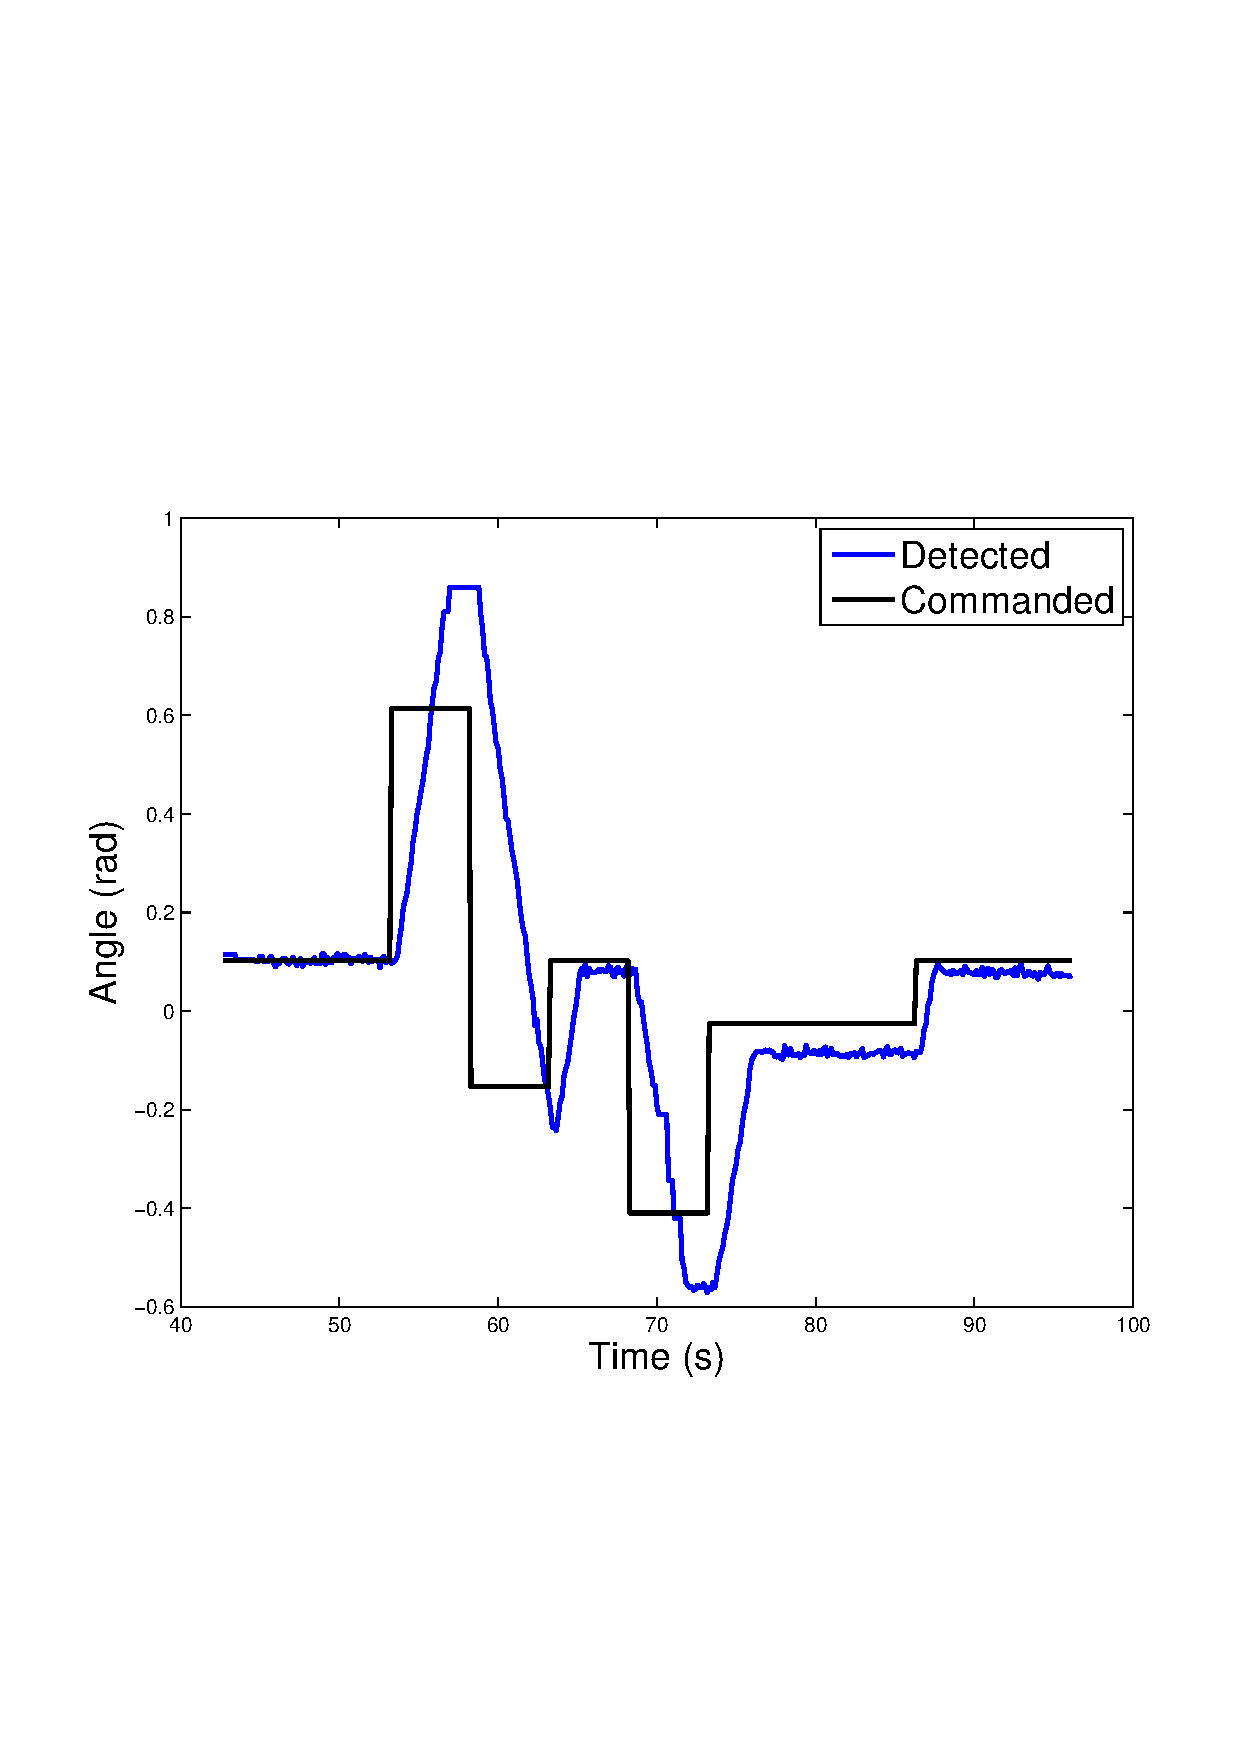
\includegraphics[width=.4\textwidth]{img/exp2b.png}
  \vspace{-.3in}
  \caption{Commanded and detected angles for one joint of the robotic arm in Experiment 2.}
  \label{fig:exp2}
\end{figure}

\section{CONCLUSIONS AND FUTURE WORK} \label{sec:conclusion}\label{sec:future}

In the current paper we have presented a working system that takes in raw trajectory input and produces a kinematic tree as output. The system's effectiveness is demonstrated in simulation and on real-world objects using fiducial markers for tracking, though we envision swapping out the fiducial markers for 3D feature tracking with a stereoscopic camera in the near future. The key contribution of this work is a modular framework for kinematic tree fitting applications, since nearly every stage in Figure \ref{fig:block-algo} can be replaced with alternative implementations to try different joint matching strategies; additionally, adding another joint type requires implementing only forward/inverse kinematics and a few ancillary functions.

There are many avenues for continuing research with this modular platform as a base. 

One area that invites inquiry is better object tracking: that using a stereoscopic camera we can achieve real-time position and orientation tracking without using fiducial markers. This requires an RGBD sensor to track features over time (perhaps using SIFT or similar techniques) and determine their orientation in 3D space. Using unsupervised feature extraction rather than manual tagging also exemplifies the need for rigid subcluster elimination (see Section \ref{sec:algorithm}). One intriguing direction, given a stationary camera, is to directly use motion for feature tracking and segmentation.

Another avenue is to re-examine the feedforward nature of Figure \ref{fig:block-algo}. Other popular vision algorithms, such as SLAM, use probabilistic structures to keep track of a belief state about the world, which in turn informs the interpretation of new sensor data. Figure \ref{fig:block-algo} might benefit from more loops, so that a speculative kinematic tree is built from initial data, which can make it easier to interpret new data (for instance, by refining the motion model of a Kalman filter). We could even incorporate a structure akin to a particle filter in order to track multiple kinematic tree hypotheses \cite{Thrun2002}.

Looking further ahead, it is somewhat limiting to confine the modeling effort to software. Humans and animals routinely modify the environment to test hypotheses and ease perception. Robots may nudge, squeeze, pick up or even throw and drop objects in order to learn about their kinematic and dynamic properties. The ``Ripley'' robotic arm system described in \cite{Hsiao2005} performs these exploratory manipulations. Applied to articulated objects, this kind of ``interactive perception'', where the current belief state of the kinematic tree determines the most informative manipulator action, could be very helpful.

In conclusion, the system presented here is modular and extensible, and we see many interesting directions for extendings its functionality.


\section{APPENDIX}

\subsection{Gradient of the Objective Function} \label{sec:gradient}
If we regard $L(\xse{u},\xse{v})$ as a chain of nested functions
\begin{align}
  L(\xse{u},\xse{v}) &= c*g(h(k(\xse{u}, \xse{v}))) + d*m(n(\xse{u}, \xse{v}))
\end{align}
then we can find the Jacobians individually
\begin{alignat*}{3}
  g(x) &= ||x||_F^2 \quad\quad& \mathbb{R}^{3 \times 3} &\rightarrow \mathbb{R} \\
  h(x) &= \log{x} \quad\quad& \mathbb{R}^{3 \times 3} &\rightarrow \mathbb{R}^{3 \times 3} \\
  k(\xse{u},\xse{v}) &= \xmat{u}_R^T \xmat{v}_R \quad\quad& SE(3) &\rightarrow \mathbb{R}^{3 \times 3} \\
  m(x) &= ||x||^2 \quad\quad& \mathbb{R}^3 &\rightarrow \mathbb{R} \\
  n(\xse{u},\xse{v}) &= \xvec{u}_T - \xvec{v}_T \quad\quad& SE(3) &\rightarrow \mathbb{R}^3
\end{alignat*}
and combine them to form the full partial derivative
\begin{align}
  \deriv{L}{\xse{u}} &= c\deriv{g}{x}\deriv{h}{x}\deriv{k}{\xse{u}} + d\deriv{m}{x}\deriv{n}{\xse{u}}
\end{align}
Checking the dimensions and using the above Jacobians, a short computation yields:
\begin{align*}
  \deriv{g}{x} &= 2x \quad\quad& 1 &\times 9 &&& % matrix cookbook p14
  \deriv{h}{x} &= x^{-1} \quad\quad& 9 &\times 9 \\
  \deriv{k}{\xse{u}} &= v_R \quad\quad& 9 &\times 16 &&&
  \deriv{m}{x} &= 2x \quad\quad& 1 &\times 3 \\
  \deriv{n}{\xse{u}} &= 1 \quad\quad& 3 &\times 16
\end{align*}
\begin{align}
  \deriv{L}{\xse{u}} &= c*2h(k(\xse{u},\xse{v}))*k(\xse{u},\xse{v})^{-1}*\xmat{v}_R + d*2n(\xse{u},\xse{v}) \nonumber\\
                     &= 2c\log(\xmat{u}_R^T\xmat{v}_R)\xmat{v}_R^T\xmat{u}_R\xmat{v}_R + 2d(\xvec{u}_T-\xvec{v}_T)
\end{align}
and this will be used to speed up the gradient descent optimization (see Algorithm \ref{alg:manip-learn}).

\subsection{Source Code}
The MATLAB and C++ code underlying the algorithms described in this paper are released under the WTFPL and may be found at \texttt{http://www.alexburka.com/penn/manip}.

\section*{ACKNOWLEDGMENTS}

\begin{enumerate}
  \item Prof. Thomas Hunter (Swarthmore)
\end{enumerate}


\bibliographystyle{IEEEtran}
\bibliography{IEEEabrv,research}




\end{document}
